\chapter{Lab Equipment}\label{chap:hardware}

In the lab, there are several computers equipped with data acquisition
systems running Windows~7 with Matlab. The hardware equipment and some
software tools are manufactured by \href{http://www.quanser.com/}{Quanser
    Consulting}, a Canadian company developing real-time control systems for
education and research. This document introduces some of the hardware
equipment to be used in the labs. Familiarity with this document is needed to
perform the labs.

\section{Hardware devices}

The lab hardware consists of three components:
\begin{enumerate}
    \item data acquisition system;
    \item power module;
    \item servomotors.
\end{enumerate}

\section{Data Acquisition Board}

In order for the computer to run a controller, analog-to-digital (A/D) and
digital-to-analog (D/A) conversions are necessary. These are done using the
data acquisition and control board (DACB), which inputs the measured
signal(s) to the computer and outputs control action to the actuator in the %chktex 36
control loop.  The DACB in this lab consists of a single board: the Q2-USB,
which is made by Quanser Consulting.  Figure~\ref{fig:q2usb}
\begin{figure}[htbp]
    \centering
    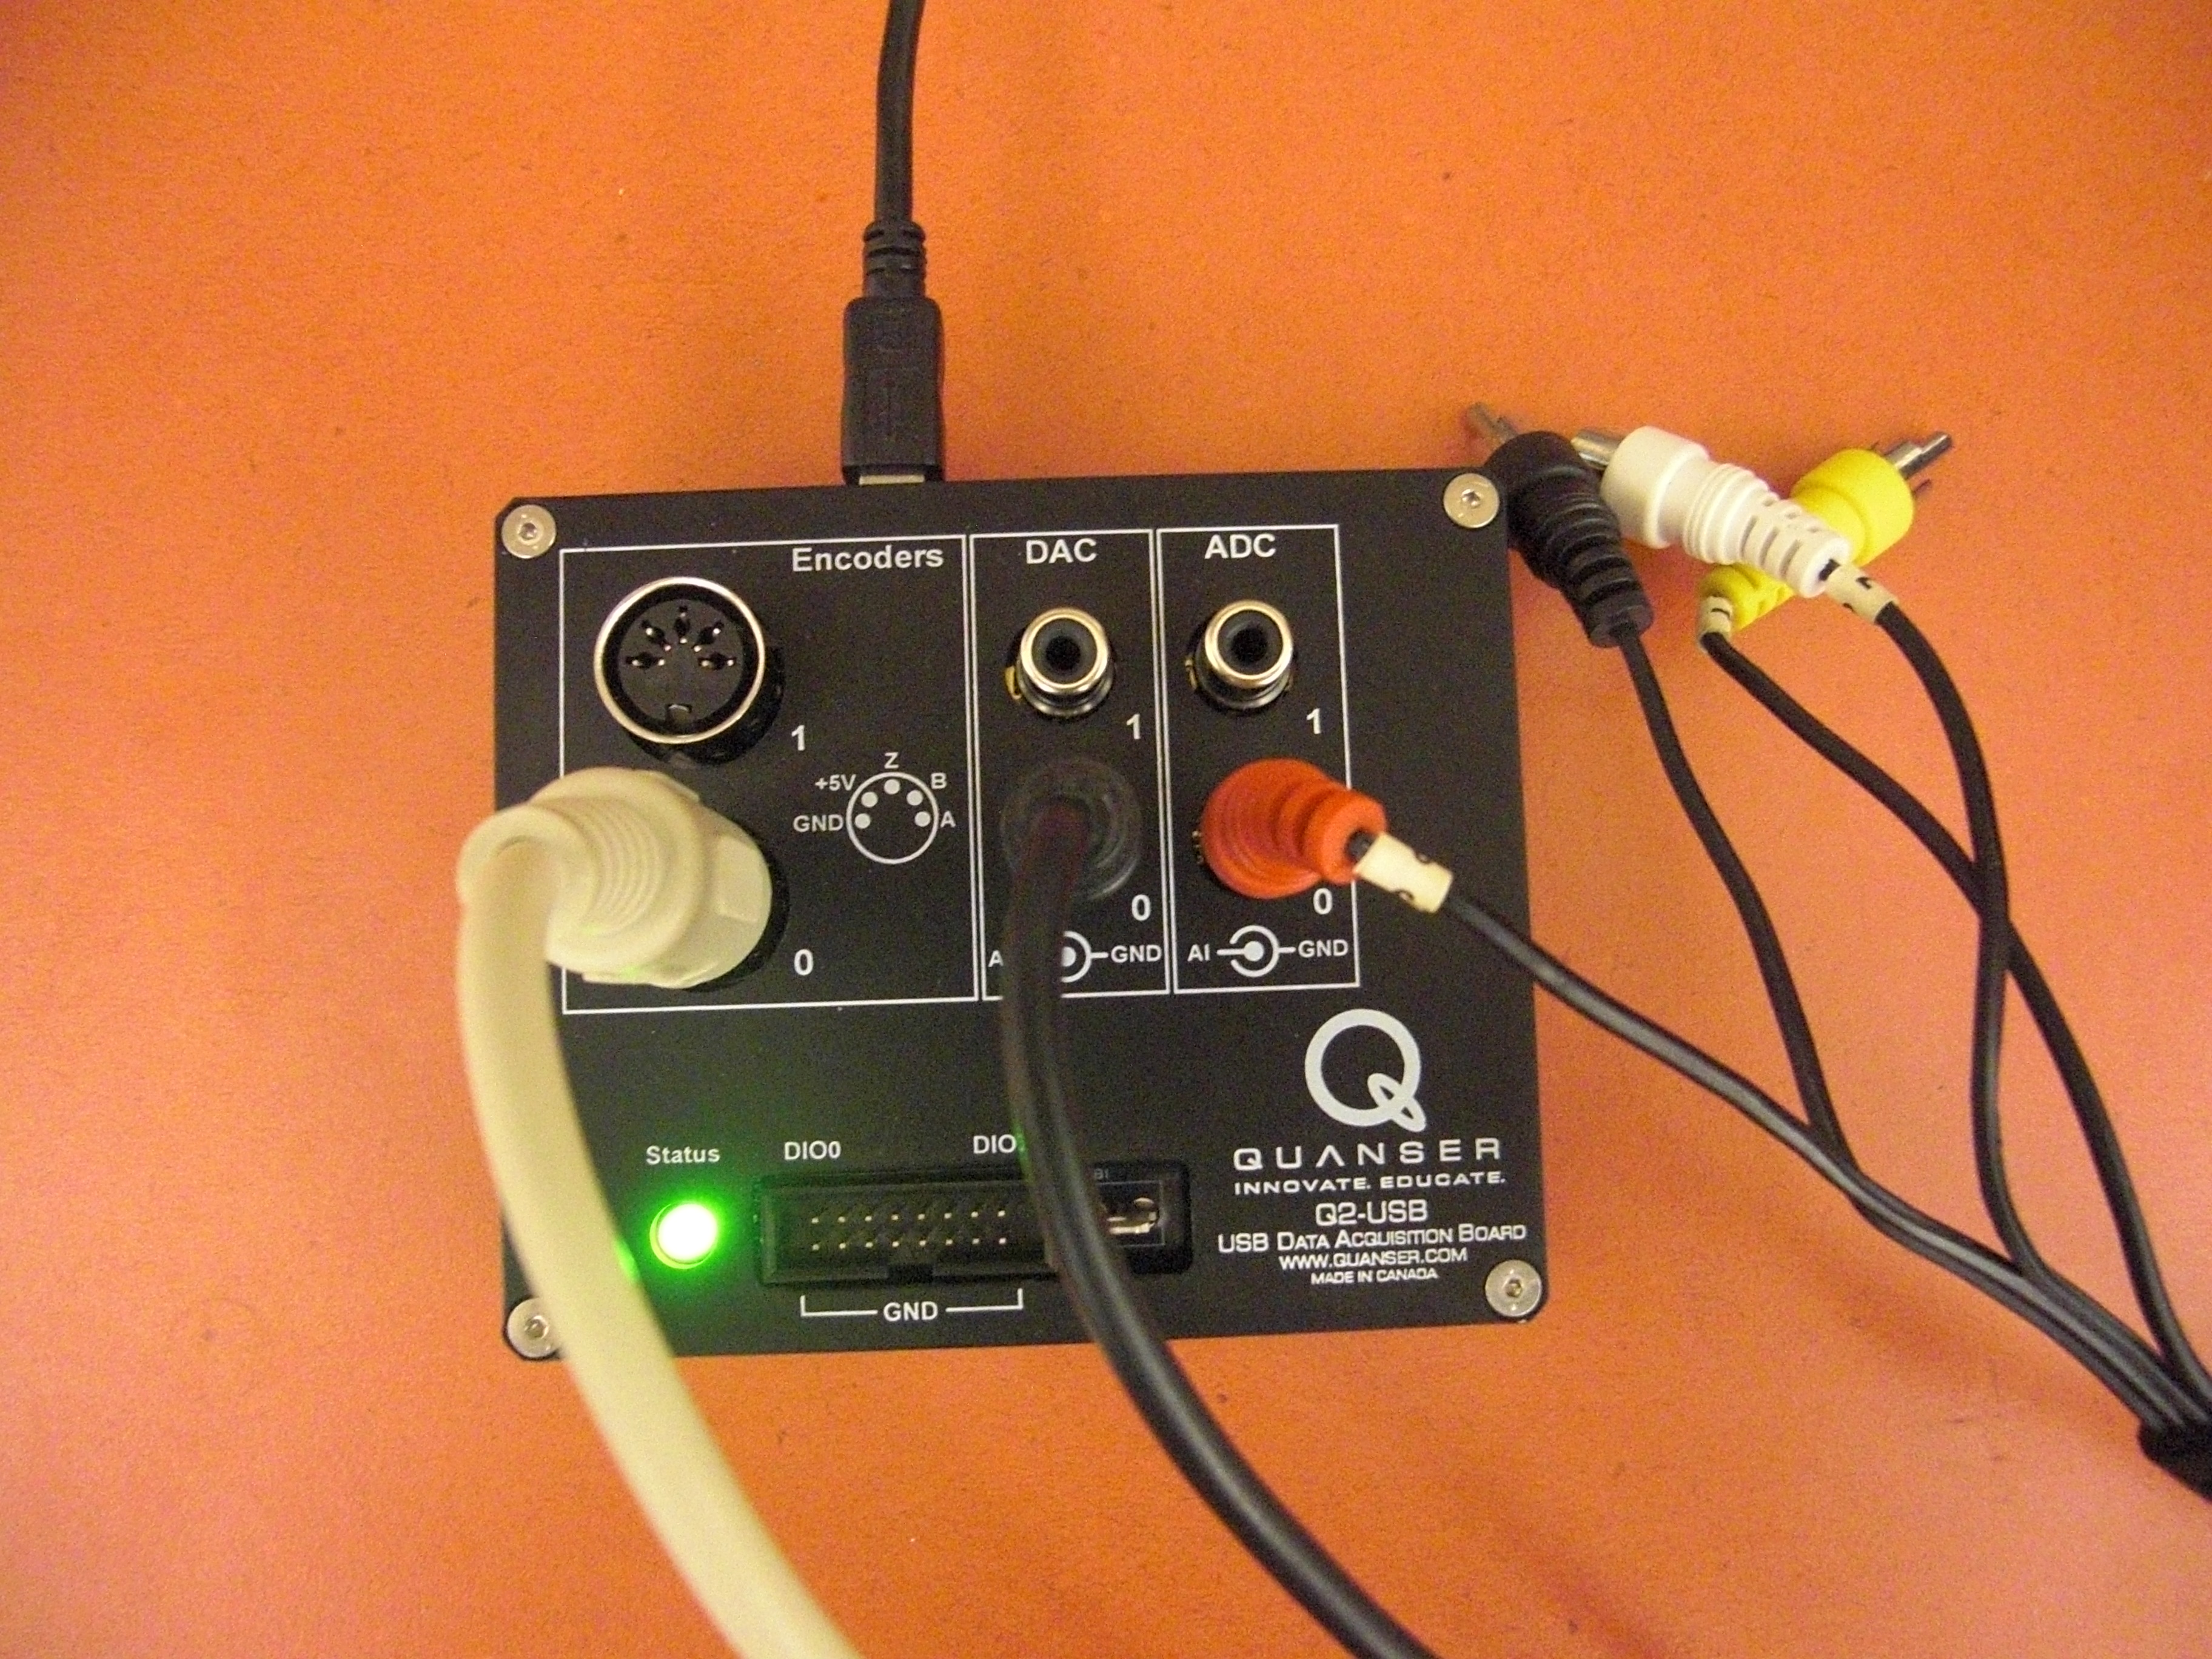
\includegraphics[width=0.6\hsize]{pix/Q2USB.jpg}
    \caption{Q2-USB data acquisition board}\label{fig:q2usb}
\end{figure}%
shows a photo of the Q2-USB card. This data acquisition board is an external
board connected to the computer through a USB port.

Figure~\ref{fig:q2usb} also shows the proper configuration of the data
acquisition board.  The Encoder is the 5~pin Din and is plugged in to
channel~0 in the Encoders portion of the board. The tachometer (S3 on the
Quanser) is the red RCA plug and is plugged into channel~0 is the ADC
portion of the board.  Finally the analog output is the solo black RCA plug
and is plugged in to channel~0 of the DAC portion of the board.

\section{Universal power module}

The universal power module (UPM-2405), which is shown in
Figure~\ref{fig:power}\@,
\begin{figure}[htbp]
    \centering
    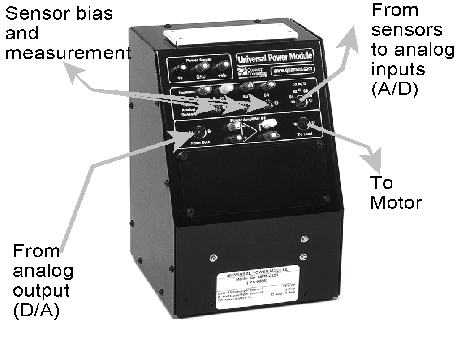
\includegraphics[width=0.6\hsize]{pix/power.jpg}
    \caption{Universal power module}\label{fig:power}
\end{figure}%
is a linear power operations amplifier. The Q2-USB data acquisition board
cannot deliver enough power to the actuators used in this lab; therefore, a
signal buffer is needed.  The UPM-2405 is used as our signal buffer since it
can deliver up to 5A~to an actuator in a non-inverting, unity gain
configuration.

The following connections can be made to/from the UPM (see the labels on the
UPM).
\begin{itemize}
    \item From analog sensors: there are four (S1-S4 inputs which can be
          connected from analog sensors (and then subsequently to the computer); the
          cable used is a 6-pin mini-din/6-pin mini-din cable (light tan colour), which
          is now referred to as the analog sensor cable.

    \item To A/D:\@ the four analog sensor signals (S1-S4) can then be connected to
          the Q2-USB terminal board for A/D conversion into the computer; the cable
          used is a 5-pin din-stereo/4RCA cable (black colour), which is now referred to
          as the A/D cables.

    \item From D/A:/@ this is where you input the D/A signal from the Q2-USB
          terminal board to the UPM;\@ the cable used is a 5-pin din-mono/RCA cable
          (black colour), which is now referred to as the D/A cable.

    \item To load: here you connect the amplified D/A signal to an actuator
          (e.g., servomotor); the cable used is a 7-pin din/4-pin din cable (black
          colour), which is now referred to as the load cable.  Note there are two types
          of load cables one with unity gain and another with a cable gain of 5.  Make
          sure you use the right one.

    \item Others: A few other connections are possible for convenience: e.g., a
          DC power supply on the top left provides 12 volts; the signal s from analog
          sensors S1-S4 can be easily monitored by connecting to a scope to the banana
          plug terminals.
\end{itemize}

\section{DC servomotor}

The Quanser DC servomotor (SRV02) is shown in Figure~\ref{fig:motor}\@.  A 3W
motor is mounted in a solid aluminium frame and drives a built-in Swiss-made
14.1:1 gearbox whose output drives an external gear, which is attached to an
independent output shaft that rotates in an aluminium ball-bearing block.
The output shaft is equipped with an encoder.  The external gear on the
output shaft drives an anti-backlash gear connected to a precision
potentiometer for measuring the output angle.  The external gear ratio can be
changed from 1:1 to 5:1 using different gears.  Two inertial loads are
supplied with the system in order to examine the effect of changing inertia
on motor performance.
\begin{figure}[htbp]
    \centering
    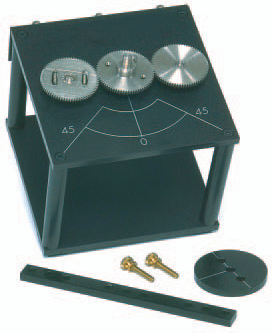
\includegraphics[width=0.6\hsize]{pix/motor-eps-converted-to.pdf}
    \caption{DC servomotor (SRV02)}\label{fig:motor}
\end{figure}%
Several connections are available for the servomotor. The input voltage
connects to the UPM using the load cable.  The potentiometer and tachometer
ports connect to the UPM-2405 using sensor cables and are used to measure
angular position and angular velocity respectively.  Additionally, the shaft
encoder port connects to the terminal board using an encoder cable and is
used to measure angular position.  The calibration factors listed in
Table~\ref{tab:conversionFactors} are needed in order to use the sensors in
units of degrees or radians.

\begin{table}[htbp]
    \centering
    \begin{tabular}{c c c }
        Connection    & Conversion (Rad)                                    & Conversion (Deg)                                   \\\bottomrule
        Encoder       & \(-\frac{2\pi}{4096}\)                              & \(-\frac{360}{4096}\)                              \\
        Tachometer    & \(\frac{100\pi}{63} \frac{\text{rad}}{\text{sec}}\) & \(\frac{18000}{63} \frac{\text{deg}}{\text{sec}}\) \\
        Potentiometer & \(\frac{1}{4096}\)                                  & \(\frac{180}{4096\pi}\)                            \\
    \end{tabular}
    \caption{Conversion factors}\label{tab:conversionFactors}
\end{table}

%%% Local Variables: 
%%% mode: latex
%%% TeX-master: "lab-manual"
%%% End: 
